\documentclass{article}
\usepackage{blindtext}
\usepackage[utf8]{inputenc}
\usepackage{amsmath,bm}
\usepackage{amstext}
\usepackage{amsfonts}
\usepackage{amsmath}
\usepackage{multirow}
\usepackage{enumerate}
\usepackage{xeCJK}
\setCJKmainfont{STKaiti}
\usepackage{algorithm}
\usepackage{algorithmic}
\renewcommand{\algorithmicrequire}{ \textbf{输入:}} %Use Input in the format of Algorithm
\renewcommand{\algorithmicensure}{ \textbf{输出:}} %UseOutput in the format of Algorithm
\usepackage{graphicx}

\title{Neural Network and Applications\\ 大作业一}
\author{陈轶洲 MF20330010}
\begin{document}
	\maketitle
	\numberwithin{equation}{section}

\section{设计方案}
本章将从两个方面介绍感知器神经网络的设计方案:
\begin{enumerate}[1)]
	\item 网络结构设计:定义网络层数,各层激活函数,输入输出及各隐藏层规模,损失函数类型;
	\item 参数设计:定义训练数据集,以及训练轮次、学习率等超参数。
\end{enumerate}

\subsection{网络结构设计}
\begin{figure}[H]
	\centering
	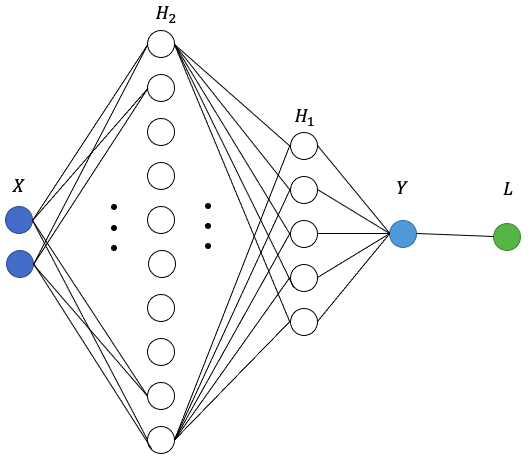
\includegraphics[scale=0.6]{neural.png}
	\caption{神经网络结构}
\end{figure}
\begin{enumerate}[1)]
	\item 网络层数:本网络除输入输出层之外,包含两个隐藏层$ H_1,H_2 $;
	\item 激活函数:通过实验对比Sigmoid、Relu、Tanh函数,Tanh激活函数取得了更好的效果,故模型选择Tanh作为激活函数;
	\item 神经元规模:由于待拟合函数为二元非线性函数,故输入层神经元个数为2,隐藏层$ H_1 $包含10个神经元,隐藏层$ H_2 $包含5个神经元,输出层为1个神经元;
	\item 损失函数:本模型选择均方误差作为损失函数,其计算方法如下:
	\begin{equation}
		LOSS = \sum_{i=1}^{n}(y_i-t_i)^2
	\end{equation}
\end{enumerate}

\subsection{参数设计}
\begin{enumerate}[1)]
	\item 训练数据集:在[-5,5]的区间中以0.1的步长取点,将取得的100个点作为二维矩阵的横纵坐标,从而生成10000个数据点,以这10000个点作为训练数据集;
	\item 迭代次数iters\_num:5000000
	\item 批处理batch\_size:100
	\item 学习率learning\_rate:0.0001
	\item 轮次epoch:50000
\end{enumerate}


\section{编程实现方案}
随报告提交的代码文件中包含functions.py、layers.py、neuralnet.py、main.py,分别对应本章将介绍的神经网络层、神经网络结构、模型训练三个层面的设计,下面将自底向上地介绍编程实现方案。
\subsection{神经网络层设计}
本节将介绍神经网络中各隐藏层的设计,包括其前向传播与反向传播的实现方法。(具体实现见layers.py)
\subsubsection{全连接层}
图\ref{fig2}给出了全连接层前向传播与反向传播的推导公式:\\
前向传播:$ Y=W^TX+B $\\
反向传播:$ \dfrac{\partial{L}}{\partial{X}}= W\dfrac{\partial{L}}{\partial{Y}}$,$ \dfrac{\partial{L}}{\partial{W}}= X(\dfrac{\partial{L}}{\partial{Y}})^T$,$ \dfrac{\partial{L}}{\partial{B}}= \dfrac{\partial{L}}{\partial{Y}}$
\begin{figure}[H]
	\centering
	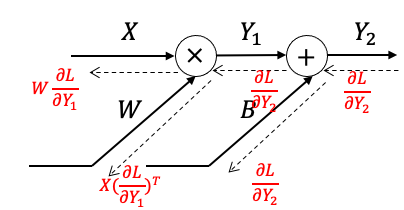
\includegraphics[scale=0.6]{FC.png}
	\caption{Fully Connected}
	\label{fig2}
\end{figure}
编程实现类$ FC() $,其包含$ forward(),backward() $两种方法,分别实现对前向传播与反向传播的计算:
\begin{figure}[H]
	\centering
	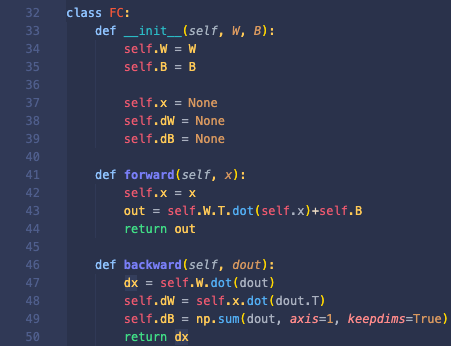
\includegraphics{fclayer.png}
	\caption{fully connection layer}
\end{figure}

\subsubsection{Relu层}
relu层的作用是将输入矩阵中的非正元素置为零,所以在前向传播中使用矩阵mask记录下所有非正元素位置,并将相应位置元素置为0。在反向传播中,再次利用mask矩阵,将传播来的偏导矩阵中的对应元素置为零。\\
下图是通过编程实现的$ Relu() $类,其包含$ forward(),backward() $两种方法:
\begin{figure}[H]
	\centering
	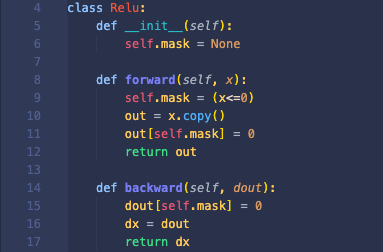
\includegraphics{relulayer.png}
	\caption{relu layer}
\end{figure}

\subsubsection{Tanh层}
tanh激活函数的计算与求导如下所示:\\
\begin{equation}
\begin{aligned}
	tanh(x) &= \frac{e^{x}-e^{-x}}{e^{x}+e^{-x}}\\
	tanh'(x) &= 1 - tanh^2(x)
\end{aligned}
\end{equation}
通过上式实现类$ Tanh() $:
\begin{figure}[H]
	\centering
	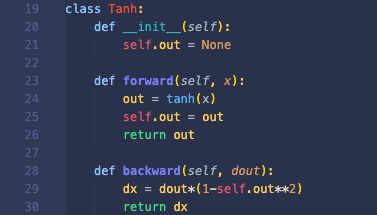
\includegraphics{tanhlayer.png}
	\caption{tanh layer}
\end{figure}

\subsubsection{Loss层}
本网络采用均方误差作为损失函数,故损失函数层的计算与求导如下所示:
\begin{equation}
	\begin{aligned}
		loss(y) &=  (y-t)^2\\
		loss'(y) &= 2(y-t)
	\end{aligned}
\end{equation}
通过上式实现$ Loss() $类:
\begin{figure}[H]
	\centering
	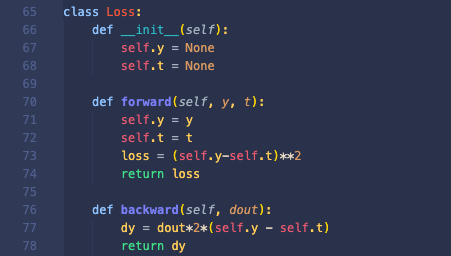
\includegraphics{losslayer.png}
	\caption{loss layer}
\end{figure}

\subsection{神经网络结构}
通过上节实现了各隐藏层的功能,本节将介绍如何通过已有的隐藏层完成神经网络类$ ThreeLayerNet() $的实现。(具体实现见neuralnet.py)

\subsubsection{初始化}
功能:对神经网络模型必要的参数,如隐藏层、激活函数等进行初始化。\\
实现方法:首先定义字典params用来保存全连接层中的权重矩阵与偏置,接着定义字典layers保存神经网络需要的各层。为了方便后续反向传播的计算,将layers定义为OrderdDict():
\begin{figure}[H]
	\centering
	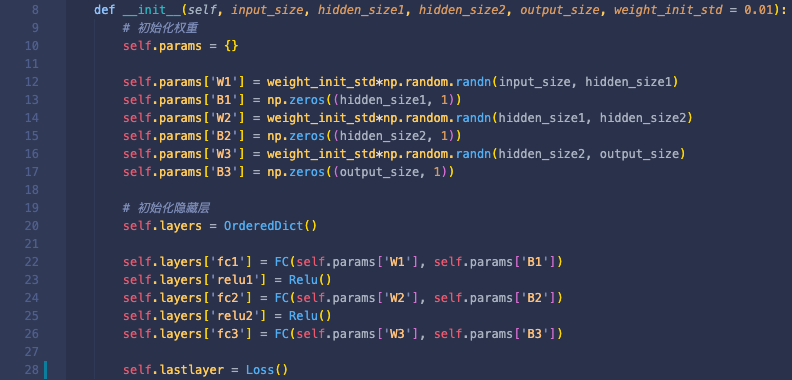
\includegraphics[scale=0.6]{init.png}
	\caption{inital}
\end{figure}

\subsubsection{predict方法}
功能:对输入数据进行预测并返回预测结果。\\
实现方法:得到输入数据后,依次调用各层的forward()方法,同时将输出作为下一层的输入,依次传递:
\begin{figure}[H]
	\centering
	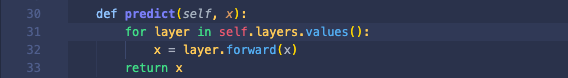
\includegraphics[scale=0.6]{predict.png}
	\caption{predict}
\end{figure}

\subsubsection{loss方法}
功能:计算模型当前的误差。\\
实现方法将中间输出输入到Loss()层中即可计算出模型的误差:
\begin{figure}[H]
	\centering
	
\includegraphics[scale=0.6]{loss.png}
	\caption{loss}
\end{figure}

\subsubsection{gradient方法}
功能:计算反向传播时损失函数对各隐藏层参数的偏导并返回。\\
实现方法:首先调用loss()方法求出模型误差,接着利用字典layers的有序性,使用reverse()方法将字典中各层的顺序反转,然后利用各层的backward()方法将dout传递下去。最后利用字典grads将各层的偏导保存并返回:
\begin{figure}[H]
	\centering
	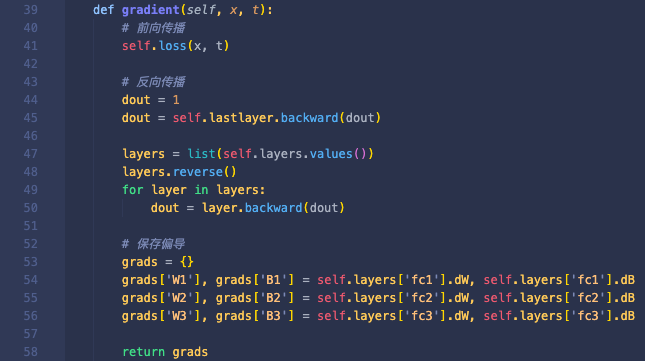
\includegraphics[scale=0.6]{gradient.png}
	\caption{gradient}
\end{figure}

\subsection{模型训练}
本节将介绍如何训练模型。(具体实现见main.py)\\
利用batch处理方法,每次从数据集中随机选择100个样本作为神经网络的输入,接着计算其输出与标签的误差,并将误差进行反向传播。在每个epoch完成后后记录模型的损失加入到列表train\_loss\_list中,直至训练结束。
\begin{figure}[H]
	\centering
	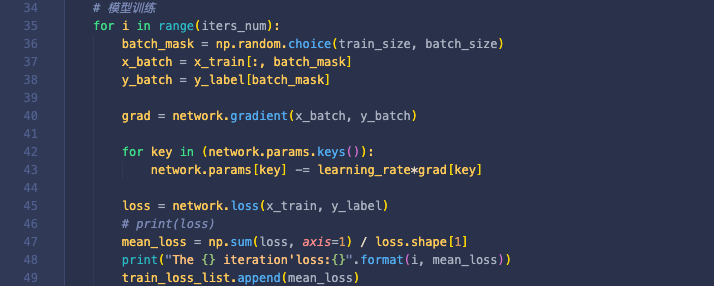
\includegraphics[scale=0.6]{train.png}
	\caption{train}
\end{figure}

\section{实验结果展示}
利用训练数据完成50000个epoch的训练后,模型的误差如下:
\begin{figure}[H]
	\centering
	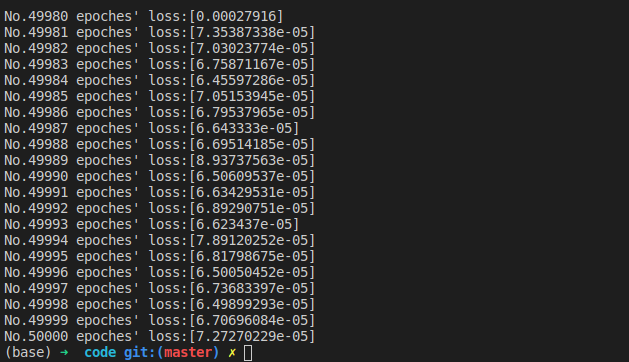
\includegraphics[scale=0.6]{result.png}
	\caption{result}
\end{figure}

训练过程中的损失函数记录如下,模型已训练至收敛:
\begin{figure}[H]
	\centering
	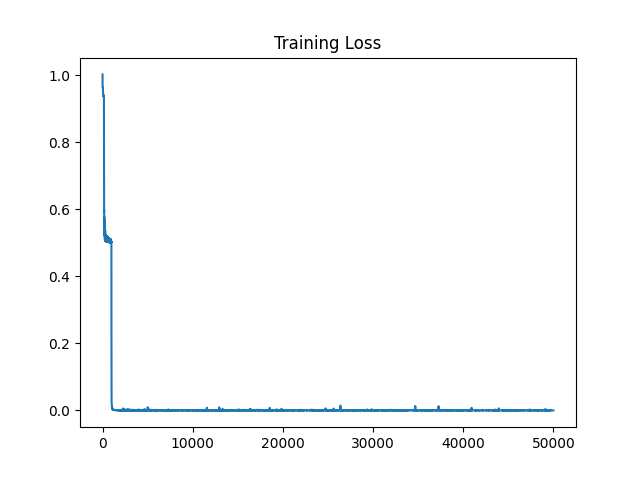
\includegraphics[scale=0.8]{tanh_5.png}
	\caption{train loss list}
\end{figure}

利用三维图像显示模型训练前与训练后的拟合差别:
\begin{figure}[H]
	\centering
	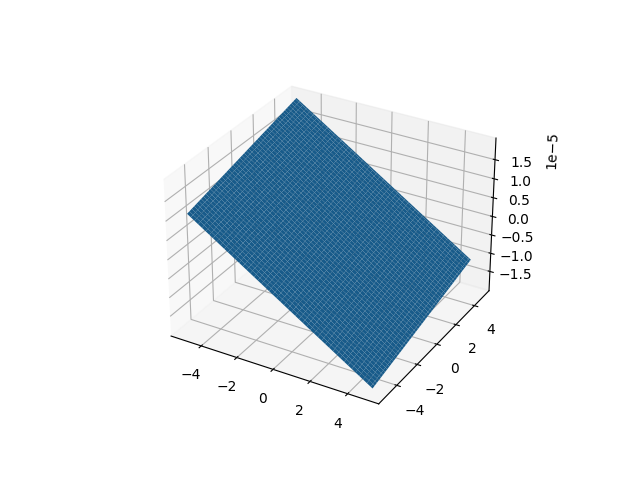
\includegraphics[scale=0.6]{3d1.png}
	\caption{before training}
\end{figure}

\begin{figure}[H]
	\centering
	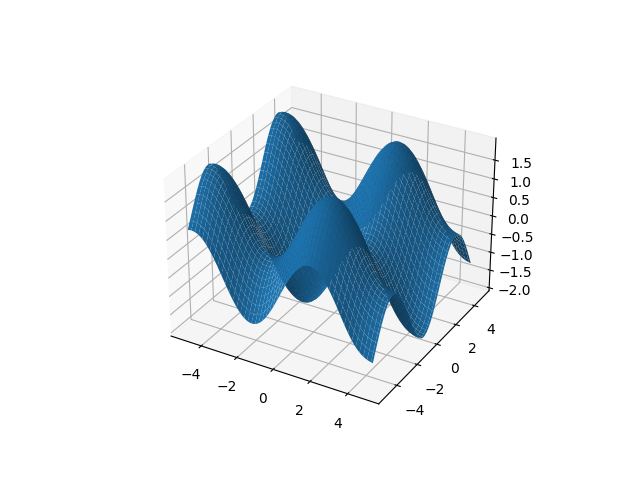
\includegraphics[scale=0.6]{3d2.png}
	\caption{after training}
\end{figure}

\section{分析与总结}
通过上一章的实验结果展示,该神经网络已经具备了拟合二元非线性函数$ y=sin(x_1)-cos(x_2) $的能力。其之所以能够拟合非线性曲线,原因在于:
\begin{enumerate}[1)]
	\item 单神经元只具有拟合线性函数的功能,单层中的多个神经元拥有拟合不同线性函数的功能。延伸至多隐藏层的神经网络,将各线性函数的加权和进行反复迭代可以达到拟合非线性函数的效果;
	\item 仅利用权重矩阵与偏置,拟合效果往往并不理想,所以需要利用激活函数。本神经网络模型采用的激活函数为tanh,它具有整流的作用,能够更好地提取函数非线性部分的特征,弱化其它不重要的特征。并且tanh的值域与待拟合函数的值域相同,均为$ [-2, 2] $,进一步提升了拟合效果,这一优势是relu、sigmoid激活函数所不具备的。
\end{enumerate}

\section{参考资料}
[1]https://zhuanlan.zhihu.com/p/47519999

\end{document}
